\documentclass[a4paper,12pt]{article}

% ==========================================
% PAQUETES Y CONFIGURACIÓN
% ==========================================
\usepackage[utf8]{inputenc}
\usepackage[T1]{fontenc}
\usepackage[spanish]{babel}
\usepackage{graphicx}
\usepackage{caption}
\usepackage{float}
\usepackage{hyperref}
\usepackage{xcolor}
\usepackage{geometry}
\usepackage{parskip}
\usepackage{booktabs}
\usepackage{array}
\usepackage{listings}
\usepackage{pgfplots}
\usepackage{amsmath}

\pgfplotsset{compat=1.18}

\geometry{
    left=2.5cm,
    right=2.5cm,
    top=2.5cm,
    bottom=2.5cm
}

\hypersetup{
    colorlinks=true,
    linkcolor=black,
    urlcolor=blue
}

\renewcommand{\arraystretch}{1.25}

% ==========================================
% CONFIGURACIÓN DE CÓDIGO
% ==========================================
\lstset{
    language=C++,
    basicstyle=\ttfamily\small,
    keywordstyle=\bfseries,
    commentstyle=\itshape,
    numbers=left,
    numberstyle=\tiny,
    stepnumber=1,
    numbersep=8pt,
    frame=single,
    breaklines=true,
    showstringspaces=false,
    tabsize=2
}

% ==========================================
% DOCUMENTO
% ==========================================
\begin{document}

%-------------------------------------------------------------------------------
% Portada
%-------------------------------------------------------------------------------
\begin{titlepage}
    \centering

    {\bfseries\LARGE
    UNIVERSIDAD NACIONAL DE SAN AGUSTÍN DE AREQUIPA
    \par}

    \vspace{0.2cm}

    {\scshape\LARGE
    Ciencia de la Computación
    \par}

    \vspace{1cm}

    {
\includegraphics[width=0.4\textwidth]{Escudo_UNSA.png}\par}

    \vspace{1cm}

    {\Large
    Computación Paralela y Distribuida
    \par}

    \vspace{0.5cm}

    {\bfseries\scshape\LARGE
    Evaluación del desempeño de algoritmos y comportamiento de la memoria caché
    \par}

    \vspace{1cm}

    {\Large
    Presentado por:
    \par}

    \vspace{0.2cm}

    {\Large
    Fabricio Jesús Huaquisto Quispe
    \par}

    \vfill

    {\Large
    Docente:
    \par}

    {\Large
    Alvaro Henry Mamani Aliaga
    \par}

    \vfill

    {\bfseries\Large
    Perú, Arequipa 2026
    \par}

\end{titlepage}

\section{Análisis de bucles anidados}

\subsection{Implementaciones}

Se implementaron dos órdenes para realizar el producto matriz--vector
\(\mathbf{y}=A\mathbf{x}\). En ambas versiones la matriz tiene tamaño
\(n\times n\), el vector de entrada tiene tamaño \(n\) y el vector de salida
se inicializa en cero. La diferencia entre las versiones es el orden de los
bucles que recorren filas y columnas.

\begin{lstlisting}[caption={Orden por filas: \texttt{row-major}},label={lst:row-major}]
for (std::size_t row = 0; row < matrix_size; ++row) {
  for (std::size_t column = 0; column < matrix_size; ++column) {
    vector_y[row] += matrix_a[row][column] * vector_x[column];
  }
}
\end{lstlisting}

\begin{lstlisting}[caption={Orden por columnas: \texttt{column-major}},label={lst:column-major}]
for (std::size_t column = 0; column < matrix_size; ++column) {
  for (std::size_t row = 0; row < matrix_size; ++row) {
    vector_y[row] += matrix_a[row][column] * vector_x[column];
  }
}
\end{lstlisting}

\subsection{Número de iteraciones y complejidad}

Para cada versión, el bucle externo se ejecuta \(n\) veces y el bucle interno
se ejecuta \(n\) veces por cada iteración del bucle externo. Por tanto, el
cuerpo de la operación matriz--vector se ejecuta exactamente

\[
T(n)=\sum_{i=0}^{n-1}\sum_{j=0}^{n-1}1=n^2
\]

veces. La complejidad temporal de ambas implementaciones es
\(\Theta(n^2)\), y el espacio adicional utilizado por el cálculo es
\(\Theta(n)\), sin contar el almacenamiento de la matriz.

\begin{table}[H]
    \centering
    \caption{Iteraciones del cuerpo para diferentes tamaños.}
    \label{tab:loop-iterations}
    \begin{tabular}{r r r}
        \toprule
        \(n\) & Iteraciones del bucle externo & Iteraciones del cuerpo \(n^2\) \\
        \midrule
        64   & 64   & 4\,096 \\
        256  & 256  & 65\,536 \\
        1\,024 & 1\,024 & 1\,048\,576 \\
        4\,096 & 4\,096 & 16\,777\,216\\
        16\,384 & 16\,384 & 268\,435\,456\\
        \bottomrule
    \end{tabular}
\end{table}

\subsection{Resultados experimentales}

Cada tiempo corresponde a la mediana de tres ejecuciones del núcleo medido,
sin incluir la creación ni el llenado de las matrices. 

\begin{table}[H]
    \centering
    \caption{Tiempo de ejecución del producto matriz--vector.}
    \label{tab:loop-times}
    \begin{tabular}{r r r}
        \toprule
        \(n\) & \texttt{row-major} (s) & \texttt{column-major} (s) \\
        \midrule
        64   & 0.000002381 & 0.000001999 \\
        256  & 0.000044124 & 0.000033215 \\
        1\,024 & 0.000839735 & 0.001767697 \\
        4\,096 & 0.011261255 & 0.120011213 \\
        16\,384 & 0.232982623 & 4.257951217 \\
        \bottomrule
    \end{tabular}
\end{table}

\subsection{Análisis del comportamiento}

A pesar que ambas implementación tienen una complejidad algorítmica de $n^2$, la ejecución muestra que una clara distinción entre los tiempos. Esto se debe a que la implementación \texttt{row-major} recorre los elementos de una fila secuencialmente aprovechando la localidad espacial al ser guardado toda una fila en caché, mientras que \texttt{column-major} recorre por columnas desaprovechando los datos cargados en caché al hacer saltos entre filas.

\section{Multiplicación clásica de matrices}

\subsection{Implementación}

La implementación calcula \(C=A\times B\), donde las tres matrices son
cuadradas de tamaño \(n\times n\). Los elementos se inicializan con valores
entre \(1\) y \(n^2\), y la medición comprende únicamente los tres bucles de
multiplicación.

\begin{lstlisting}[caption={Tres bucles de la multiplicación clásica}]
for (std::size_t row = 0; row < matrix_size; ++row) {
  for (std::size_t column = 0; column < matrix_size; ++column) {
    for (std::size_t inner = 0; inner < matrix_size; ++inner) {
      matrix_c[row][column] +=
          matrix_a[row][inner] * matrix_b[inner][column];
    }
  }
}
\end{lstlisting}

\subsection{Iteraciones y complejidad}

El cuerpo del algoritmo se ejecuta

\[
T(n)=\sum_{i=0}^{n-1}\sum_{j=0}^{n-1}\sum_{k=0}^{n-1}1=n^3
\]

veces. Cada iteración realiza una multiplicación y una suma. La complejidad
temporal es \(\Theta(n^3)\) y el espacio ocupado por las tres matrices es
\(\Theta(n^2)\).

\begin{table}[H]
    \centering
    \caption{Iteraciones del producto interno en la multiplicación clásica.}
    \label{tab:classic-iterations}
    \begin{tabular}{r r r}
        \toprule
        \(n\) & Elementos de cada matriz & Iteraciones \(n^3\) \\
        \midrule
        64  & 4\,096  & 262\,144 \\
        128 & 16\,384 & 2\,097\,152 \\
        256 & 65\,536 & 16\,777\,216 \\
        512 & 262\,144 & 134\,217\,728 \\
        1\,024 & 1\,048\,576  & 1\,073\,741\,824 \\
        \bottomrule
    \end{tabular}
\end{table}

\subsection{Resultados experimentales}

\begin{table}[H]
    \centering
    \caption{Tiempo de ejecución de la multiplicación clásica.}
    \label{tab:classic-times}
    \begin{tabular}{r r r}
        \toprule
        \(n\) & Iteraciones \(n^3\) & Tiempo (s) \\
        \midrule
        64  & 262\,144       & 0.000160147 \\
        128 & 2\,097\,152    & 0.000902168 \\
        256 & 16\,777\,216  & 0.009696666 \\
        512 & 134\,217\,728 & 0.113081077 \\
        1\,024 & 1\,073\,741\,824 & 1.431647785 \\
        \bottomrule
    \end{tabular}
\end{table}

\subsection{Relación entre tamaño y tiempo}

Al tener una complejidad $n^3$, al duplicar el tamaño de $n$, la cantidad de operaciones se multiplica por $8$, pero por optimizaciones del sistema y caché, se consigue un incremento aproximado de $5.63$ entre $n = 64$ y $n = 128$, pero estas optimizaciones decaen en tamaños de $n$ más grandes como $n=512$ y $n=1024$ donde se obtiene un incremento aproximado de $12.66$, por encima del teórico $8$, esto debido que por la gran cantidad de datos, estos no caben completamente en los niveles de caché más rápidos.

\section{Multiplicación de matrices por bloques}

\subsection{Fundamento e implementación}

La multiplicación por bloques particiona las filas y columnas de las matrices
en submatrices de tamaño máximo \(b\times b\). Para cada combinación de
bloques se calcula la contribución parcial de un bloque de \(C\):

\[
C_{I,J}\mathrel{+}=A_{I,K}B_{K,J}.
\]

Los límites de los bloques se recortan con
\(\min(\text{inicio}+b,n)\), por lo que el algoritmo también funciona cuando
\(b\) no divide exactamente a \(n\). La implementación utiliza seis bucles
anidados: tres para seleccionar los bloques y tres para recorrer sus elementos.

\begin{lstlisting}[caption={Seis bucles de la multiplicación por bloques}]
for (std::size_t block_row = 0; block_row < matrix_size;
     block_row += block_size) {
  const std::size_t row_end =
      std::min(block_row + block_size, matrix_size);
  for (std::size_t block_column = 0; block_column < matrix_size;
       block_column += block_size) {
    const std::size_t column_end =
        std::min(block_column + block_size, matrix_size);
    for (std::size_t block_inner = 0; block_inner < matrix_size;
         block_inner += block_size) {
      const std::size_t inner_end =
          std::min(block_inner + block_size, matrix_size);
      for (std::size_t row = block_row; row < row_end; ++row) {
        for (std::size_t column = block_column; column < column_end;
             ++column) {
          for (std::size_t inner = block_inner; inner < inner_end; ++inner) {
            matrix_c[row][column] +=
                matrix_a[row][inner] * matrix_b[inner][column];
          }
        }
      }
    }
  }
}
\end{lstlisting}

\subsection{Iteraciones y complejidad}

El número de combinaciones de bloques es
\(\lceil n/b\rceil^3\). La suma de las iteraciones de los tres bucles internos
para todas las combinaciones de bloques es exactamente \(n^3\), incluso cuando
el último bloque de una dimensión es parcial. Por ello, la complejidad temporal
general sigue siendo \(\Theta(n^3)\), mientras que el almacenamiento de las
matrices sigue siendo \(\Theta(n^2)\).

\begin{table}[H]
    \centering
    \caption{Configuraciones de bloques y número de combinaciones de bloques.}
    \label{tab:block-iterations}
    \begin{tabular}{r r r r}
        \toprule
        \(n\) & \(b\) & \(\lceil n/b\rceil\) & Combinaciones \(\lceil n/b\rceil^3\) \\
        \midrule
        64  & 8  & 8 & 512 \\
        64  & 16 & 4 & 64 \\
        128 & 16 & 8 & 512 \\
        128 & 32 & 4 & 64 \\
        256 & 32 & 8 & 512 \\
        256 & 64 & 4 & 64 \\
        512 & 64 & 8 & 512 \\
        512 & 128 & 4 & 64 \\
        1\,024 & 128 & 8 & 512 \\
        1\,024 & 256 & 4 & 64 \\
        \bottomrule
    \end{tabular}
\end{table}

\subsection{Resultados experimentales}

\begin{table}[H]
    \centering
    \caption{Tiempo de ejecución con distintos tamaños de bloque.}
    \label{tab:blocked-times}
    \begin{tabular}{r r r r}
        \toprule
        \(n\) & \(b\) & Iteraciones aritméticas \(n^3\) & Tiempo (s) \\
        \midrule
        64  & 8  & 262\,144       & 0.000132902 \\
        64  & 16 & 262\,144       & 0.000115722 \\
        128 & 16 & 2\,097\,152    & 0.000869885 \\
        128 & 32 & 2\,097\,152    & 0.001011389 \\
        256 & 32 & 16\,777\,216  & 0.006659205 \\
        256 & 64 & 16\,777\,216  & 0.006959075 \\
        512 & 64 & 134\,217\,728 & 0.070591367 \\
        512 & 128 & 134\,217\,728 & 0.112277331 \\
        1\,024 & 128 & 1\,073\,741\,824 & 0.617179742 \\
        1\,024 & 256 & 1\,073\,741\,824 & 0.605565270 \\
        \bottomrule
    \end{tabular}
\end{table}

\subsection{Comparación con la multiplicación clásica}

Apesar de que ambas implementaciones mantienen una misma complejidad algorítmica de $n^3$, la múltiplicación por bloques aprovecha de mejor manera la memoria caché al trabajar con trozos pequeños que sí llegan a entrar por completo en los niveles más rápidos de la memoria caché. Esta mejora se puede ver más claro en el caso de $n=1024$ donde tenemos una mejora clara de $\sim44\%$.

\section{Movimiento de datos y memoria caché}

\subsection{Patrones de acceso}

En la implementación clásica, la matriz $A$ presenta un patrón favorable de acceso, ya que $A[row][inner]$ recorre consecutivamente los elementos de una fila. Esto permite aprovechar la localidad espacial. Por el contrario, $B[inner][column]$ recorre una columna de $B$, generando accesos separados. Este patrón puede ocasionar un número elevado de fallos de caché. El elemento $C[row][column]$, en cambio, se reutiliza durante todas las iteraciones del bucle interno, presentando una elevada localidad temporal. \\

En la implementación por bloques, los accesos se restringen temporalmente a subregiones de $A$, $B$ y $C$. Una vez que un bloque ha sido cargado en caché, múltiples operaciones pueden reutilizar sus datos antes de avanzar hacia otro bloque. De esta manera se reduce la necesidad de recuperar repetidamente datos desde niveles más lentos de la jerarquía de memoria.

\subsection{Localidad espacial y temporal}

La localidad espacial se manifiesta cuando el algoritmo accede consecutivamente a elementos cercanos en memoria. \\

La localidad temporal aparece cuando un dato cargado recientemente vuelve a utilizarse antes de ser expulsado de la caché.

\subsection{Relación entre cómputo y movimiento de datos}

El desempeño de un algoritmo no depende únicamente del número de operaciones aritméticas. Cada operación requiere que sus operandos estén disponibles en registros o en niveles rápidos de memoria. Cuando un dato no se encuentra en caché, debe recuperarse desde un nivel inferior de la jerarquía de memoria, introduciendo una latencia adicional.

\section{Evaluación utilizando Valgrind y KCachegrind}

\subsection{Procedimiento}

Los perfiles se generaron con Cachegrind mediante los objetivos definidos en el
\texttt{Makefile}. Para esta evaluación se utilizó un tamaño de matriz de
\(n=1024\), comparando la implementación clásica con dos configuraciones de
multiplicación por bloques:

\begin{lstlisting}[language=bash,caption={Comandos para generar y visualizar perfiles}]
make cachegrind-multiply-matrix SIZE=1024
make cachegrind-multiply-matrix-blocked SIZE=1024 BLOCK=128
make cachegrind-multiply-matrix-blocked SIZE=1024 BLOCK=256

make kcachegrind-multiply-matrix
make kcachegrind-multiply-matrix-blocked
\end{lstlisting}

Cachegrind simuló una caché L1 de instrucciones de 32 KiB, una caché L1 de
datos de 48 KiB y una caché de último nivel de 12 MiB, con líneas de 64 bytes.
Los valores presentados corresponden a ejecuciones con \(n=1024\). En la
columna de referencias de datos se consideran conjuntamente las lecturas y
escrituras realizadas durante la ejecución.

\begin{table}[H]
    \centering
    \caption{Contadores de Cachegrind para \(n=1024\).}
    \label{tab:cachegrind}
    \scriptsize
    \begin{tabular}{l r r r r r r r}
        \toprule
        Implementación &
        Tiempo (s) &
        I refs &
        I1 misses &
        D refs &
        D1 misses &
        LLi misses &
        LLd misses \\
        \midrule

        Clásica &
        54.026 &
        9\,691\,652\,271 &
        2\,276 &
        4\,303\,112\,590 &
        1\,348\,466\,446 &
        2\,205 &
        977\,672 \\

        Bloques \(b=128\) &
        31.093 &
        9\,838\,914\,767 &
        2\,283 &
        4\,342\,112\,999 &
        141\,120\,994 &
        2\,211 &
        1\,108\,228 \\

        Bloques \(b=256\) &
        36.769 &
        9\,758\,865\,294 &
        2\,281 &
        4\,320\,986\,732 &
        167\,687\,934 &
        2\,210 &
        1\,411\,157 \\

        \bottomrule
    \end{tabular}
\end{table}

\subsection{Capturas de KCachegrind}

\begin{figure}[H]
    \centering
    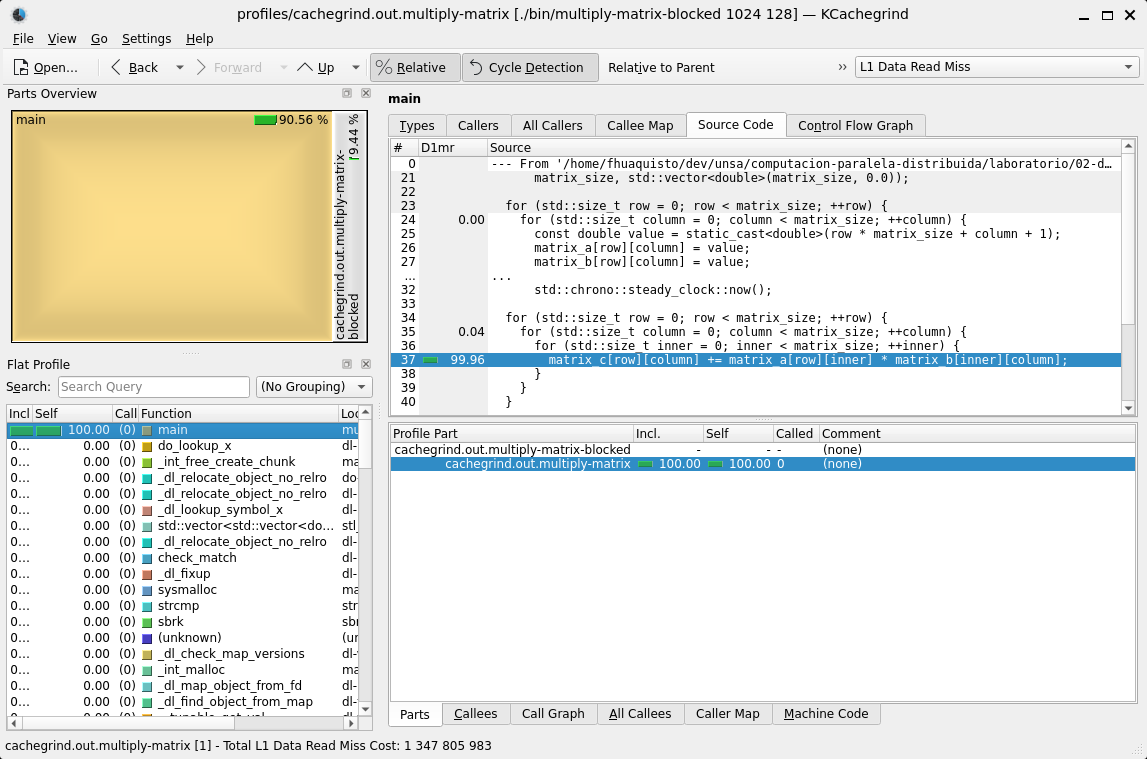
\includegraphics[width=1\linewidth]{kcachegrind.png}
    \caption{Comparación de los fallos de lectura en caché L1 para la
multiplicación clásica y la multiplicación por bloques con \(n=1024\)
y \(b=128\), utilizando Cachegrind y KCachegrind.}
\end{figure}

\subsection{Análisis crítico}

En la imagen se muestra que la mayor parte de los fallos de lectura en la caché L1 se concentra en la operación principal de multiplicación y acumulación de elementos de las matrices. La implementación clásica representa aproximadamente el $90.6\%$ de los fallos, mientras que la implementación por bloques con $b=128$ representa solo un $9.4\%$. Esto evidencia el mejor aprovechamiento de la localidad de datos.

\section{Repositorio del código fuente}

El código fuente, el archivo de construcción, las instrucciones de uso y los
perfiles disponibles se encuentran en el siguiente repositorio público:

\begin{center}
\url{https://github.com/fhuaquistoq/unsa/tree/main/computacion-paralela-distribuida/laboratorio/02-desempeno-algoritmos}
\end{center}

El repositorio contiene las implementaciones de los dos órdenes de bucles, la
multiplicación clásica, la multiplicación por bloques, el \texttt{Makefile}, el
\texttt{README.md} y los perfiles de Cachegrind.

\end{document}
